\subsection{MetaQC}
MetaQC package provides an objective and quantitative tool to help determine the inclusion/exclusion of studies for meta-analysis. More specifically, MetaQC provides users with six quantitative quality control (QC) measures: including IQC, EQC, AQCg, CQCg, AQCp and CQCp. Details of how each measure is defined and computed can be found in \cite{kang2012metaqc}. In addition, visualization plots and summarization tables are generated using principal component analysis (PCA) biplots and standardized mean ranks (SMR) to assist in visualization and decision. 
``MetaQC" package itself can be downloaded at (\url{https://github.com/metaOmics/MetaQC}). 
\subsubsection{Procedure}

\begin{figure}[H]
\begin{center}
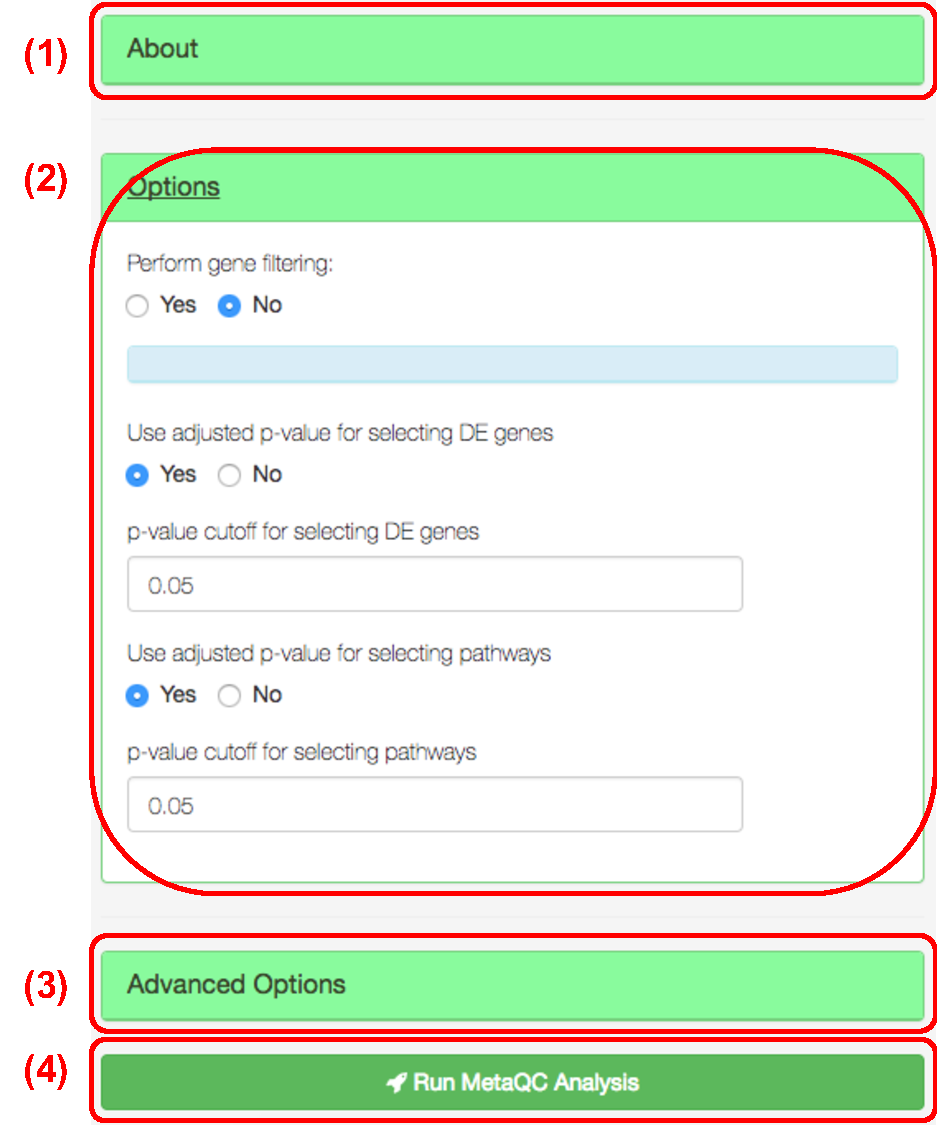
\includegraphics[scale=0.5]{./figure/metaQC/metaQCoption.pdf}
\caption{``MetaQC" options}
\label{fig:MetaQCoption}
\end{center}
\end{figure}
There are three main options available for the ``MetaQC" package as shown in Figure~\ref{fig:MetaQCoption}. 
The complete list of MetaQC options are available in Section~\ref{sec:completeList_MetaQC}.

\begin{steps}
\item \textbf{Options:}
Under the drop-down menu ``options" (Figure~\ref{fig:MetaQCoption} {\color{red}(2)}),
users can 

\begin{itemize}
\item perform gene filtering. Gene filtering is suggested to reduce computational cost. Once ``Yes" is chosen for gene filtering, 
users need to further specify the filtering cutoffs by mean and variance. 
In the demo example, 
the merged data have already had gene filtering in the merging step, so no further filtering is performed. 
\item specify the approach (either by raw p-value or adjusted p-value) and cutoff to select potentially DE genes needed in the computation of IQC, EQC, AQCg and CQCg.
\item specify the approach (either by raw p-value or adjusted p-value) and cutoff to select potentially enriched pathways needed in the computation of AQCp and CQCp.
\end{itemize}
Note that the larger the p-value or adjusted p-value is, 
the more genes will be included in the quality control computing.
The default parameters are suggested for the purpose of MetaQC.

\item \textbf{Advanced options:}



Under the drop-down menu ``Advanced Options" ({\color{red}(3)} in Figure~\ref{fig:MetaQCoption}), users are allowed to tune other parameters of MetaQC.
In particular, it includes the selection of pathways by pathway size and the number of permutations to run to obtain the six measures. 
A detailed list of all options available for the package can be found in Section~\ref{sec:completeList_MetaQC}. 
However, this is advanced options and users are suggested not to modify the option setting in this section without knowing the method. 

\item \textbf{Run MetaQC Analysis:}

Once all the above options are specified, users can click on ``Run MetaQC Analysis" (Figure~\ref{fig:MetaQCoption}  {\color{red}(4)}  ) to implement the tool. 

\end{steps}



\subsubsection{Results for MetaQC on AML example}

\begin{figure}[H]
\begin{center}
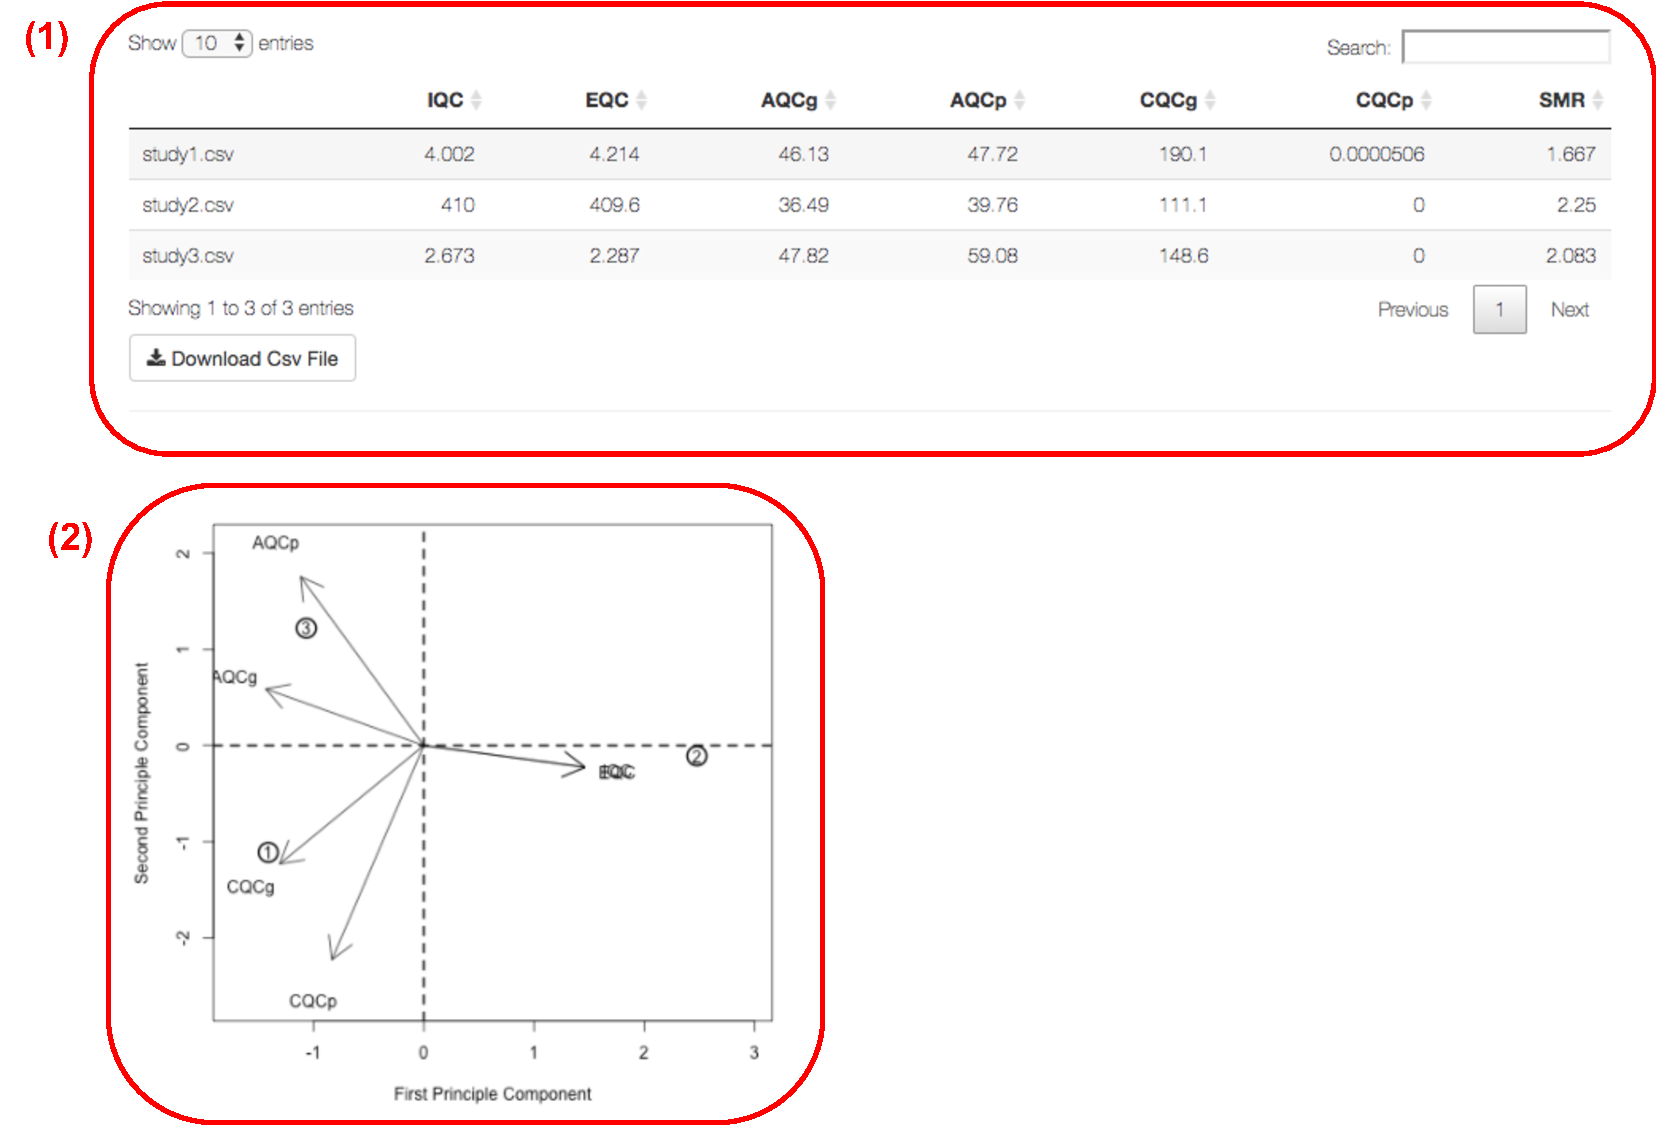
\includegraphics[scale=0.65]{./figure/metaQC/metaQCresult_AML.pdf}
\caption{``MetaQC" Results for AML example.
Figure~\ref{fig:MetaQCresult_AML} {\color{red} (1)} includes seven columns, 
with the first six columns corresponding to the six quantitative quality control measures of all studies (a larger value indicates a better quality) and the seventh column is the rank summary statistics of all the six quality measures (a lower rank indicates a better quality). 
Users can download the full table as a csv file by clicking on ``Download Csv File". 
In addition to the tabular results, ``MetaQC" also generated a PCA biplot based on the six quality control measures, 
where the circled number is the study index and arrows indicate different measures. 
If a study (a circled number) is along the direction of majorities of the six QC direction, then the study has higher quality and consistent with other studies.
In generally, studies with larger SMR values, and studies more off from the other studies and a majority of the measures are considered lower quality.
In this specific example, since the six QC direction are quite heterogeneous, 
we cannot exclude any study because of quality issue.
}
\label{fig:MetaQCresult_AML}
\end{center}
\end{figure}


The performance of ``MetaQC" in the AML example is shown in Figure~\ref{fig:MetaQCresult_AML}.
Detailed descriptions of these studies can be found in Table~\ref{tab:realDataLeukemia}. 
As shown in Figure \ref{fig:MetaQCresult_AML}, 
MetaQC module generates a summary table of MetaQC results (\ref{fig:MetaQCresult_AML} {\color{red} (1)} ) 
as well as a PCA biplot (\ref{fig:MetaQCresult_AML} {\color{red} (2)}). 
Since the AML example has very good data quality,
we won't be able to demonstrate how to use MetaQC to identify studies of low quality.
Thus, in order to demonstrate how to give suggestions on excluding studies with low quality or incompatibility with other studies,
we further performed ``MetaQC" on the prostate cancer example.

\subsubsection{Results for MetaQC on prostate cancer example}




\begin{figure}[H]
\begin{center}
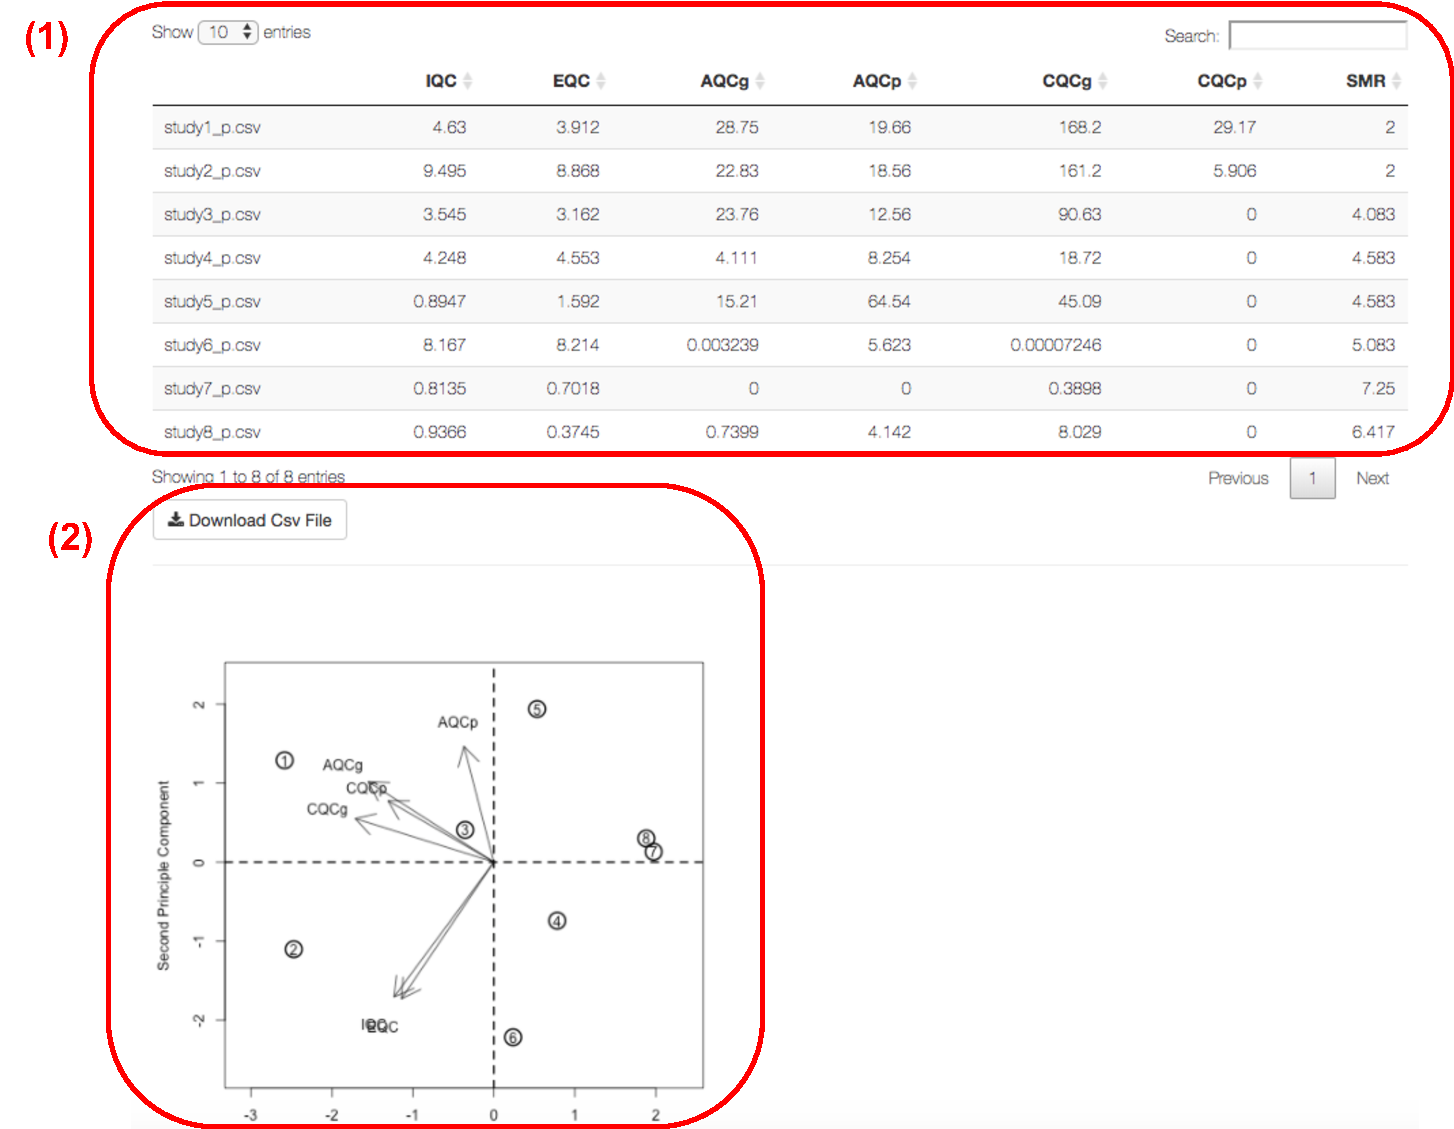
\includegraphics[scale=0.65]{./figure/metaQC/metaQCresult_Prostate.pdf}
\caption{``MetaQC" Results for prostate cancer example.
Figure~\ref{fig:MetaQCresult} {\color{red} (1)} includes seven columns, 
with the first six columns corresponding to the six quantitative quality control measures of all studies (a larger value indicates a better quality) and the seventh column is the rank summary statistics of all the six quality measures (a lower rank indicates a better quality). 
Users can download the full table as a csv file by clicking on ``Download Csv File". 
In addition to the tabular results, ``MetaQC" also generated a PCA biplot based on the six quality control measures, 
where the circled number is the study index and arrows indicate different measures. 
If a study (a circled number) is along the direction of majorities of the six QC direction, then the study has higher quality and consistent with other studies.
In generally, studies with larger SMR values, and studies more off from the other studies and a majority of the measures are considered lower quality.
In this specific example, since the six QC directions all direct to left, 
and study 8 and study 7 are discordant with this direction.
As a consequence, study 8 and study 7 are inconsistent with other studies and suggested to be removed from the meta-analysis.
}
\label{fig:MetaQCresult}
\end{center}
\end{figure}


The test data used to demo the ``MetaQC" package here is merged from eight prostate cancer studies with 30\% of genes filtered out by mean and 30\% filtered out by variance (2077 genes remained for the MetaQC analysis). 
Detailed descriptions of these studies can be found in Table~\ref{tab:realDataProstate}. 
As shown in Figure~\ref{fig:MetaQCresult}, 
MetaQC module generates a summary table (Figure~\ref{fig:MetaQCresult} {\color{red} (1)}) of MetaQC results 
as well as a PCA biplot (Figure~\ref{fig:MetaQCresult}  {\color{red} (2)}). 
In this specific example, the 7th and the 8th studies have larger SMR values than the other studies.
In addition, in the biplot,  the 7th and the 8th studies are inconsistent with the six QC direction.
Therefore, both the 7th and the 8th studies have relatively poorer quality, and they are inconsistent with other studies.
Users should pay attention to these potential outlier-studies.


